\chapter{The Programming Model}
\label{chp:programming}

The previous chapter has examined the application of retroaction in 
event-sourced systems. We described conceptual considerations and challenges 
which emerge from this combination. Furthermore, we examined two very 
different architectures which utilize retroaction. The objective of this 
chapter is to illustrate how a programming model for the unified architecture 
can work. For this, we outline an appropriate programming model and its 
prototypical implementation.

%=====================
\section{System Model}
We describe the \emph{outline} of a programming model and make many simplifying 
assumptions in order to focus on relevant concepts. 
The objective of our programming model is to illustrate how retroaction in 
event-sourced systems can work. We do not claim to lay out a programming model 
which withstands challenges such as performance, scalability, parallelization, 
or distribution.
We make the assumption that the programming model runs in a single-threaded 
environment with one timeline, that sufficient resources are available, and
that no error handling is required.
In the remainder of this chapter, the term \emph{runtime engine} is used when 
referring to the system which provides underlying functions (such as the 
persistence of events). We will not deepen details of such a runtime engine, 
since this is not subject of this work. The code examples in this chapter are 
written in the scripting language JavaScript. They are excerpts from our 
prototypical implementation, which is detailed in the second part of this 
chapter. The code examples have in most cases been shortened to focus on the 
concepts, but they are otherwise in correspondence to our implementation.

\section{Primitives of Retroaction}
The objective of the programming model outlined in this chapter, is to provide 
programmers with access to an application's history in the programming 
environment. We aim for the possibility of modifying and interacting with the 
application's history retroactively in a single environment.
The primitives of retroaction which we require for this are:
 
\pagebreak

\begin{enumerate}
	\item \emph{Branching:}
	It needs to be possible to create a branch at a certain branching point 
	in the timeline. The subsequent timeline from this point on is copied to 
	the branch and can be modified.
	Modifications on the branch do not affect the timeline.
	Through the specification of a branching point, the retroactive operations 
	can be restrained to the part of the timeline from the branching point on.

	\item \emph{Access to Prior States:}
	The application can access its own history and the history of branches.

	\item \emph{Interaction with Branches:}
	The state of branches can be queried and results from computations on 
	branches integrated back into the timeline.

	\item \emph{Delete/Insert Commands or Events:}
	Specified commands or events can be retroactively deleted or inserted.

	\item \emph{Exchange Command Processing:}
	The command processing implementation can be retroactively exchanged
	and evaluated by replaying the application's command history.
\end{enumerate}

For our further considerations we build upon the principles of the unified 
architecture described in Section \ref{sec:arch:arch-unified} and illustrated 
in Figure \ref{fig:embedded} (both on page \pageref{fig:embedded}).
%
In short, we retain the overall CQRS architecture with a segregated command and 
query model. Commands are issued from an application layer and result in events, 
which are published to the query model. In commands, developers have access to 
retroactive operations. 
They can create branches, as well as insert (or delete) commands and events.
The only mean to read state is by issuing queries.
%
A close coupling of queries and subsequent, dependent command to the actual 
CQRS interface is discouraged for the higher application logic.


%=====================
\subsection{Events}
\subsubsection{Events as State Modifications}
\label{sec:events-as-statem}

In a strictly event-sourced architecture, events are viewed as \emph{implicit}
changes to an abstract system state (e.g. \texttt{AddedProductToCart(id=533)}). 
In order to derive the current state of the application (e.g. the list of items 
in the shopping cart), state has to be constructed by interpreting events.
%
For our programming model we propose a different point of view: 
system state as an object, accessed and modified by commands. Events are created 
by an underlying runtime engine after modifications have been applied; they 
contain the modifications which were applied to the state object. The event is 
created by the runtime engine, which computes the differences to the prior state 
object.
%
This point of view eases us to record which persisted events and commands in
the timeline possess a causal relationship, by annotating commands with the
information which properties of the state objects were used to compute the state 
modification. Among other things, tracking these dependencies can be used to 
determine what needs to be replayed after a retroactive modification has been 
applied (Section \ref{sec:dependent}). 
This can be achieved by tracing which state properties in the future are affected 
by a retroactive modification.
A retroactively inserted command \texttt{AddProductToCart} could e.g. require 
the recomputation of a subsequent \texttt{PlaceOrder} command, in order to keep 
the timeline consistent.
Similarly, when removing an event, all causally dependent events can be removed 
as well. This can prevent issues of causality violations (e.g. temporal paradoxes). 

The following algorithm can be used to compute the causally related events to a 
selected event. The underlying concept is that a causal relationship exists when 
the computation of an event has built on a prior event.
The algorithm is initialized with a selected event and returns all forward 
events in the timeline, which have a causal relationship with it.

\begin{enumerate}
	\item Lookup which state properties were modified during the computation 
	of \cmd{selectedEvent}. Save those as \cmd{modifiedProperties}. Create 
	an empty array \cmd{causalityTrace}.

	\item Examine the subsequent event in the timeline (\cmd{nextEvent}), 
	until the algorithm returns or the end of the timeline is reached: 
		\begin{itemize}
			\item Was \cmd{nextEvent} computed by reading any of these \cmd{modifiedProperties}? 

			\begin{itemize}
				\item Yes? The event has a direct causal
				relationship to \cmd{nextEvent}, add the event to \cmd{causalityTrace}.
				To find the indirect causally dependent events, apply this algorithm recursively for \cmd{nextEvent}.

				\item No? Check if the computation of
				\cmd{nextEvent} modified any of the \cmd{modifiedProperties}.
				\begin{itemize}
					\item Yes? The computation replaced certain properties without reading anything
					originally used by \cmd{selectedEvent}.
					These properties can then be removed from \cmd{modifiedProperties}, since 
					subsequent events will not have a causal relationship to \cmd{selectedEvent} 
					based on these properties. The next step is to check, if there are any properties left in \cmd{modifiedProperties}.
					\begin{itemize}
						\item Yes? Process to the next event in the timeline.
						\item No? The algorithm returns its results.
					\end{itemize}
					\item No? Process to the next event in the timeline.
				\end{itemize}
			\end{itemize}

		\end{itemize}
\end{enumerate}


\subsubsection{Capture State Changes in Events}
\label{sec:capturing-changes}
Events capture state changes to the system state object.
In the context of retroaction, the form in which state changes are recorded 
(i.e. the delta encoding) is important to consider. The delta encoding heavily
impacts the possibilities of retroaction. Let us examine two options how 
data differences can be encoded: Unix diffs and JSON Patches.

In Unix, the \texttt{diff} tool can be used to output differences between two 
files. This output can be used to transform matching parts of a file using e.g. 
the \texttt{patch} tool. Both tools are commonly used for software development 
and utilize basically this format:

\begin{lstlisting}[style=stylec]
-state.shoppingCart = [1, 2, 3];
+state.shoppingCart = [1, 2, 3, 4];
\end{lstlisting}

This so called ``diff'' describes the difference from one file to another on a 
line-by-line basis. Diffs are commonly applied to replace parts of one file 
(the ones prefixed with ``\texttt{-}'') with other parts (prefixed with 
``\texttt{+}''). 
%
Thus, the diff can only be applied to exactly the first line, prefixed with 
``\texttt{-}''. If we modify line 1 of the original file to 
``\texttt{state.shoppingCart = [0, 1, 2, 3]}'', the above patch then could no 
longer be applied to the file, since line 1 of the above diff would no longer 
match the file. This is a desirable behavior when working with source code, 
where minor differences can have a big impact.

For retroaction, however, a different behavior can be more appropriate. If we 
introduce a retroactive change, it is desirable to retain the possibility of 
applying all subsequent changes (i.e.  diffs or patches) in the timeline.
For example, adding an id to the above \cmd{shoppingCart} array in the original 
file should not annihilate previously created patches which are placed later in 
the timeline. If these later patches add other products to the cart it would be 
desirable to retain the possibility of still applying them.
%
This can be achieved by capturing the \emph{operations} which were applied to 
the state object. A technology which uses such a mechanism are JSON Patches 
\cite{RFC6902}. They encode modifications to JavaScript objects and provide 
the ability to rebuild the state of an object by applying these modifications 
successively. 
%
The JSON Patches specification defines six operations which can be applied to 
properties of objects. Among them are operations which encode that properties 
were added, removed, replaced, or moved. 
Transferred to the above example, an according JSON Patch can be of this form:

\begin{lstlisting}[style=styled]
{ "op": "add", "path": "/state/shoppingCart/-", "value": 4 }
\end{lstlisting}

The ``\texttt{-}'' suffix in this case specifies that the value 4 is appended
to the array \texttt{state.shoppingCart}. In this case, changes to the original 
file do not conflict with the patch -- it can still be applied.
But the issue is not solved completely; in the case of direct value assignments 
to a variable, or the direct modification of a value at a certain index in the 
array, the patch still annihilates retroactive modifications. This is not 
necessarily an issue, but it can have a limiting impact on retroactive modifications.
%
In Section \ref{sec:rap}, we describe how retroaction-aware programming can be 
utilized to mitigate this issue. For the programming model in this chapter we 
focus on \emph{events as recordings of the operations behind state changes}, 
as used by JSON Patches.

\subsection{Commands}
We apply the view on commands as described for CQRS (Chapter \ref{chp:background}): 
commands as requests to invoke a certain logic. This decoupling enables us to 
separate intended modifications from the command processing implementation which 
they trigger.
Separating these concerns enables us to retroactively replace the command processing 
implementation at an arbitrary point in the timeline and reprocess commands with a
different processing implementation. This allows for the observation of alternate 
application states.

In our programming model, the runtime engine splits ``external'' requests into 
a series of multiple ``internal'' commands. 
%
The commands in this series then are sequentially processed. After the processing 
of a command is finished, the runtime engine checks if it succeeded. Therefore the 
processing function returns information on its success or failure.
If the processing succeeded, an event is computed and persisted to the timeline. 
Next, the subsequent command in the series is processed. If the command failed, 
the commands in the series will not be processed further. But the subsequent 
commands -- which were not invoked -- are still persisted to the timeline. 
This serves the purpose of enabling later command replays. 

The resulting event from a command processing is created by the underlying runtime 
engine. This event contains modifications of the state object which occurred during 
the command processing. Together with the command which triggered the processing, 
it is appended to the timeline. 
%
This concept follows our conceptual considerations from Section \ref{sec:replaying-se}:
We argued that it is important for expressive retroaction to view side effects as 
isolated, for they can be controlled individually in a replay.
Furthermore, we argued that each of the commands must be persisted in the timeline, 
independent of their failure or success. %This making them available for replays. 

In the programming model in this chapter, a developer writes individual processing 
functions for each command. \mbox{Listing \ref{lst:ecmd}} displays the processing 
of a simplified command. The depicted command applies a discount to an order, and 
annotates what it used for its computation. 
Furthermore, the command and the resulting event are tagged. These tags can be 
used to reference commands or events (e.g. for removals or as branching points).
The concept of tagging commands and events will be detailed in Section \ref{sec:tags} 
of this chapter.

\begin{lstlisting}[
	style=styled, 
	caption=Example of a command.,
	label = lst:ecmd
]
commands.tags.applyDiscount = ["discount-modifications"];

commands.applyDiscount = function(request, state) {
	/* find the total order price in the global state object */
	var totalPrice = state.orders[request.orderId].totalPrice;

	/* apply 10% discount */
	state.orders[request.orderId].discount = totalPrice * 0.1;

	/* if the order is changed retroactively at a past point this 
	   command needs to be replayed, since a different discount 
	   would then be computed */
	var readDuringComputation = [ 
		"state.orders[" + request.orderId + "].totalPrice"
	];

	/* specify tags for this event */
	var eventTags = ["applied-discount"];

	return {
		success: true,
		newState: state,
		read: readDuringComputation, 
		eventTags: eventTags
	};
}
\end{lstlisting}


\subsection{Retroaction}

\subsubsection{Scope of Branches}
\begin{figure}
	\centering
	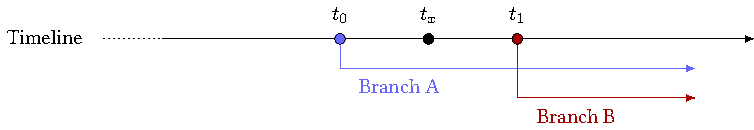
\includegraphics[width=0.95\textwidth]{../illustrations/nested-branches.pdf}
	\caption{
		The figure depicts a scenario, in which branches exist as part of the system state.
		The system at $t_0$ creates a branch A at an arbitrary former point. Branch A
		exists from then on within the system state (i.e. the timeline). At $t_1$, a 
		further branch B, with its branching point at $t_x$, is created. 
		Branch B then contains the \emph{nested} Branch A.
	}
	\label{fig:nested-branches}
\end{figure}

There are a number of possibilities concerning the duration of a branch's
existence. Two possibilities are (1) for branches to be persisted as part of 
the system's state. This enables the usage of a branch in multiple commands.
An option (2) is for branches to be only existent temporarily, during the 
processing of a single command. 

If branches are available over the course of processing multiple commands, it is
important to consider that this yields the possibility of nested branches.
Nested branches can then occur when a branch is created within a command and
succeeding commands create further branches (Figure \ref{fig:nested-branches}).
The further branches would then contain the system state -- and thus the
earlier created branches as well.
To avoid problems here, the same branch object should not be referenced in
multiple branches. Each event and command should be assigned to exactly one
branch
This allows for the coexistence of a branch in various branches. If the same 
branch object is nested in multiple branches, unforeseeable behavior can occur.
For our programming model we view branches as only temporarily existent,
for the scope of a command.
Persisting branches as part of the system state would imply that they are 
replicated to all data models. For the use cases in this chapter this is 
unnecessary.


\subsubsection{Timeline Pointers and Tags}
\label{sec:tags}
In order to enable expressive retroactive operations, it needs to be possible 
to reference points in the timeline. These \emph{timeline pointers} can then be 
used to reference events and commands as branching points, insertion marks, or 
for removal.
To achieve this, we propose the possibility of annotating events and commands 
with a list of tags. These tagged events and commands can then be used as 
pointers to locations in the timeline.

Enabling the tagging of commands \emph{and} events makes sense, since they both 
serve a different purpose. A request to invoke a command is always issued by the 
application, whereas an event describes how the system reacts to it.
The resulting event, triggered through the command, depends on the command
processing implementation of the system. Therefore it makes sense to annotate 
the resulting event with tags \emph{in the command processing}.
Annotating commands enables us to filter for commands, independent of how they
are processed. %Tagging both, commands and event, enables working with either 
tags.
%
For commands, tagging allows to dynamically exclude message categories (or 
individual messages) in replays. This can be used to exclude e.g. side effect 
afflicted operations, in order to prevent side effects from being reinvoked.

\subsubsection{Access to Retroaction}
The retroactive capabilities in our programming model can only be accessed from 
within commands -- not within queries. This characteristic adheres to the design 
of the unified architecture as described in \ref{sec:arch:arch-unified}.
In this section we examine individual operations of our API in detail.
%
In order to utilize retroaction, the first step in our programming model is 
always to create a branch of the ``main'' timeline. For this, a branching point 
needs to be specified. The following retroactive operations can be applied to 
create branch objects and gain retrospective information:

\begin{enumerate}[(i)] 
	\item \cmd{branchObject = createBranch(:tag, "before" || "after")}\\
	A branch of the timeline can be created by invoking this function within a command.
	The \cmd{:tag} is a unique tag of either a command or an event.
	By supplying ``\cmd{before}'' or ``\cmd{after}'', it is possible to specify 
	if the branching point should precede the tag or be placed after it.

	\item \cmd{stateObject = branchObject.getState()}\\
	This method can be applied to a branch object, it returns the latest state object. 

	\item 
	\cmd{eventArray = branchObject.getEvents([:tag])}\\
	Returns an array of events, which match the supplied tags.
	For each event the state of the timeline at the time of the event
	is supplied as well. This state can be accessed under the property 
	\cmd{:event.state}.
	When called on a branch object, the events are returned from this branch.
\end{enumerate}

Retroactive modifications of an application's history can be removal or insert 
operations, as well as a retroactive change of the underlying application logic 
(the command processing). 
Following our argumentation from Section \ref{sec:editing-log}, retroactive 
modifications can only be applied to branch objects.
%
Furthermore, a branch cannot apply retroactive modifications to itself.
The following operations can be used to apply modifications to the branch object:

\begin{enumerate}[(i)] 
\setcounter{enumi}{3}
	\item \cmd{branchObject.insertEvent(:tag, :event, "before" || "after",}\\
	\cmd{~~:validatorFn)}\\
	An event in the form of a JSON Patch can be inserted at a unique, tagged point.
	The validator function \cmd{:validatorFn} is optional and will
	described in more detail in this chapter.

	\item \cmd{branchObject.deleteEvents([:tag], :dependentOnes)}\\
	If \cmd{:dependentOnes} is set to true, the events which have a
	causal relationship to the ones supplied are removed as well.

	\item \cmd{branchObject.insertCommand(:tag, :command, "before" || "after")}\\
	A command can be inserted by specifying an insertion point and a command. 
	The listings in this chapter contain examples for this command.

	\item \cmd{branchObject.deleteCommands([:tag], :dependentOnes)}\\
	If commands are deleted, the respective event is deleted as well.
	Otherwise it would no longer be possible to conduct a command replay
	for a corresponding event.

	\item 
	\cmd{branchObject.changeCommandFunction(:old, :new)}\\
	\cmd{changeCommandFunction(:old, :new)}\\
	This function can be invoked either for branch objects or for the timeline. 
	It inserts a special type of ``runtime engine command-event pair'' in the
	timeline. This pair takes a special role in command and event replays. 
	It denotes that for the processing of the \cmd{:old} command, the \cmd{:new}\, 
	function should be used from this point on.
	We utilize call-by-naming for this and supply the function names as arguments. 
	It is necessary to insert a command-event pair to denote this change in the 
	processing function. Inserting solely an event, would pose an issue to command 
	replays, since this event would not be considered in a command replay.

	Another possibility for persisting changes in the command processing, is to 
	understand the command processing implementation of a system as part of the 
	state. This concept is used by the Chronograph platform and will be detailed 
	in Chapter \ref{chp:chrono}.
\end{enumerate}

Our programming model exposes additional operations, to manually trigger replays.
An alternative would be an immediate evaluation strategy, where the computation of
changes takes place immediately after e.g. an insert operation has been invoked. 
But this does not suit well, for the reasons described in Section \ref{sec:editing-log}:
using immediate evaluation in conjunction with a series of multiple retroactive
operations then leads to potentially unnecessary computations.

\begin{enumerate}[(i)] 
\setcounter{enumi}{8}
	\item \cmd{branchObject.rebuildState()}\\
	State on the branch is rebuilt based upon the persisted events.

	\item \cmd{branchObject.commandReplay([:tag])}\\
	This method triggers a replay of the commands supplied in the tags array.
	The recomputed commands yield newly computed events. For these
	``new'' events, causal dependencies to subsequent events are checked.
	If subsequent events with a direct or indirect causal relationship exist, 
	these are recursively recomputed as well (by re-processing their respective 
	commands).

	\item \cmd{branchObject.partialReplay([:reuse], [:recompute])}\\
	The \cmd{:reuse} and \cmd{:recompute} arrays contain tags.
	If causally dependent events exist, they are recomputed as well.
\end{enumerate}

The following listing (Listing \ref{lst:rexample}) depicts an example of a command 
which creates a branch, applies retroactive operations to it, and integrates results 
from the branch back into the main timeline.
The branch is encapsulated in an object, which exposes access to retroactive 
modification methods, replay mechanisms, and the branches' history, and current state.
%
It is then possible to create history-aware algorithms, which utilize the 
application's history as part of their computation. We describe examples of 
such commands in the later part of this chapter.

\begin{lstlisting}[
	style=styled,
	label=lst:rexample,
	caption = {Example command, which utilizes retroaction.}
]
var newCommandFn = function(command, state) {
	// ... 
	return { newState: ..., read: ... };
}

var exampleCommand = function(command, state) {
	/* the branch is an object which exposes retroactive operations */
	var branchingPoint = "timeline-tag0";
	var b = createBranch(branchingPoint);

	/* an event is created (in the form of a JSON Patch) and inserted */
	var evt = createEvent({"op": "add", "path": "/state/-", 
				     "value": {"name": "Alice"}});
	b.insertEvent("timeline-tag1", evt, "before");
	b.rebuildState();

	/* get the state from the branch */
	var s = b.getState();

	/* retroaction */
	b.changeCommandFunction("exampleCommand", "newCommandFn");
	b.insertCommand("footag", "AddToCart({ product: 321 })", "before");
	b.commandReplay(["AddToCart"], true);

	/* analyze state of the branches and save result */
	var s2 = b.getState();
	if (...) state.retroactiveAnalysis = ...;

	return { newState: state, read: [] };
}
\end{lstlisting}

After the function has returned, the underlying runtime engine creates an event
consisting of the command, the command's arguments, and the state modification.
This event is published to the query models and then visible to queries.

The above listing described only command and event replays.
As illustrated in Section \ref{sec:replaying-se}, the concept of partial replays 
gives us fine-grained control over when to newly compute an event and when to use 
an already persisted one. This feature can be used to control side effects.
In a partial replay, causal relationships between events are taken into
account. Thus, if only one command is replayed this has the recursive effect of
causally dependent commands being replayed as well (Section \ref{sec:replaying-se}).
For the events which are specified to be reused, the reprocessing of the
command is skipped.
Listing \ref{lst:partial-replay} illustrates how a partial replay can be conducted.

\begin{lstlisting}[
	style=styled,
	label = lst:partial-replay,
	caption = The listing depicts how a partial replay can be conducted.
]
/* newly compute the commands in this array. instead of reusing 
   the already persisted events, the command is newly invoked. 
   events which possess a causal relationship to the newly 
   resulting events are recomputed as well. */
recomputeCommands = [ "stock-price" ];

/* for the tags in the array use the persisted events instead of 
   newly processing the command */
reuseEvents= [ "stock-price" ];

/* conduct the partial replay on a branch */
var b = createBranch("timeline-tag0");
b.partialReplay({ recompute: recomputeCommands, reuse: reuseEvents });
\end{lstlisting}

\begin{comment}
The following example illustrates another example of a partial replay. Here,
commands are newly invoked and the developer specifies which commands should 
not be newly invoked:

\begin{lstlisting}[style=styled]
var exemplaryRetroactiveCommand = function(command, state) {
	/* normal command replay. besides the commands supplied, each 
	   command in the branch is invoked again. For those the already 
	   persisted event is used. If foregoing commands possess a causal 
	   relationship to the events in the supplied array, the causal 
	   relationship is ignored. */

	var b = createBranch("timeline-tag0");

	/* replay all commands, except for the tags supplied in the array, 
	   for those use the persisted events */
	b.partialReplay({ usePersistedEvents : ["mail-alerts"] });

	b.commandReplay({ replayFrom : "timeline-tag0");

	return {
		newState: state,
		read: []
	];
}
\end{lstlisting}
\end{comment}

As described in Section \ref{sec:validation}, the recordings of causal dependencies 
between events cannot only be used to recompute subsequent, causally dependent events, 
they can also be used to remove subsequent, causally dependent events. 
The following listing depicts an example of such a modification:

\begin{lstlisting}[style=styled]
var b = createBranch("timeline-tag0");
var deleteCausallyDependentOnes = true;
b.deleteEvent("some-event-reference, deleteCausallyDependentOnes);
\end{lstlisting}


\pagebreak
\subsection{Retroaction-aware Programming}
\label{sec:rap}
Programming constructs in commands can conflict with retroactive modifications.
For example, a developer might always decrement a certain state property by one in a
command processing implementation, whilst relying on some knowledge about the context 
of the application. 
An assumption could be that a value $x$ is defined as $x \in \{1,\dotso,n\}$.
The developer could apply the decrement, in order to shift the value to reference 
array indices so that $x \in \{0,\dotso,n\}$.
Through retroactive changes, this ``one off'' assumption may no longer hold and the 
decrement operation thus suddenly have a different semantics.

A first idea to cope with this issue, is to provide more semantics to certain operations. 
This can be done by providing helper functions (or an API) to the developer, in order to 
resolve the ambiguity of operations.
For example, a helper function \mbox{\cmd{ConvertToIndices}} could be provided to
developers. This function would convert numbers to array indices and
could be used instead of the decrement operation.
Thus, the intention behind the operation would be clear. In a replay, the
helper function could be adapted, in order to not break programming instructions.
Another example is the usage of \cmd{getLast()} over ``\cmd{var last = state.foo[99]}'',
where 99 is a presumed last index. 

The delta encoding of events can also be used to persist the semantics of state changes.
If the appending of a value to the just mentioned array is done whilst relying on 
the knowledge that the last element will ``always'' be 99, this could be a direct 
assignment of the form ``\cmd{state.foo[100] = 'bar'}''.
The delta encoding would then not capture that the intention was to append a value. 
An array push instruction -- e.g. ``\cmd{state.foo.push('bar')}'' -- is a better 
alternative, since this allows the runtime engine to capture that the intention was 
to append a value to the array.
There are various possibilities how the intention of a state change can be captured: 
for the developer to capture this intention manually by creating the patch by himself, 
through source code analysis, or through helper functions which provide more semantics.
The decision depends on the context of the application and either behavior can be desirable.


\subsection{Validation}
\label{sec:programming-validation}
Validation conditions can be written as a validator function. Such a validator 
function can be supplied along with the retroactive operations. 
The validator function in this case gets the state before the modification
and the state after the intended modification supplied as arguments.
The NoSQL database CouchDB uses a similar mechanism for validating changes
to documents\footnote[1]{\href{http://guide.couchdb.org/draft/validation.html}{http://guide.couchdb.org/draft/validation.html}}.
If the validation is successful (i.e. it returns \texttt{true}), the event is 
persisted to the timeline. If not successful (returns \texttt{false}), the event 
is discarded. The following listing illustrates an example of a retroactive
modification, where a validator function is supplied.

\begin{lstlisting}[style=styled]
var b = createBranch(branchingPoint);

var validatorFn = function(oldState, newState) {
	if (newState.price < 0) return false;
	else return true;
};
b.insertEvent("timeline-tag1", "{ items: 0  }", "before", validatorFn);
\end{lstlisting}

As detailed in Section \ref{sec:validation}, state mutating side effects
require special attention when validating the timeline for consistency.
They need to be delayed, until it is clear if the validation of the command's
processing results succeeded.
Otherwise, the side effect would already have occurred and could not be
revoked. This can be solved by returning an array with functions which need
to be delayed from the command processor. If the \texttt{validatorFn} succeeds, 
the functions in the array are invoked subsequently.

\begin{lstlisting}[style=styled]
var cmdWebRequest = function(cmd, state, validatorFn) {
	// ...
	var writingSideEffectFn = function () { http.post(...); };

	return {
		state: state,
		read: [],
		delayUntilValidated: [ writingSideEffectFn ]
	};
}
\end{lstlisting}

A possible scenario to apply this concept, is to retroactively reprocess a 
command which executes a reading side effect. Based on the return value, the 
command modifies the system state and executes a writing side effect. Using 
the described concept, it is possible to validate the modified state, before 
persisting the event and triggering the side effect.
%
The expressiveness of this concept is limited to simple scenarios though, but 
it provides a -- admittedly narrow -- possibility to use validation in 
combination with side effect afflicted commands.
This basic concept could be enhanced by supplying e.g. the entire branch
with all its events and commands. Other possibilities are to supply the 
command, which triggered the processing, as an argument.

\subsection{Return-values of Commands}
\label{sec:return-values}
As illustrated in Section \ref{sec:cqrs}, commands in a strict ES+CQRS 
architecture possess no return value.
%
But the opinion on the question whether commands may still return a value, is 
disputed in the CQRS domain. Some projects which apply CQRS allow for replies\footnote[1]{\href{http://rbmhtechnology.github.io/eventuate/architecture.html\#event-sourced-actors}{http://rbmhtechnology.github.io/eventuate/architecture.html\#event-sourced-actors}},
whereas authors like Greg Young promote an explicit \emph{no}: a command should 
never return a value \cite[p.17]{Young2013}. Commands are described as possessing 
a void return type. They mutate state, but do not return a value. Instead, solely 
queries can be used to gather data.
%
If commands never return anything, there is no way of knowing when a command
has been executed or when a corresponding event has been appended to the timeline.
But for certain use cases it is desirable to have this information returned
to the application. This information can be used to e.g. delay queries, until a 
certain command has been processed.

As we view it, the overall intention behind th no-return value nature of
commands, is to prevent bilateral commands which return \emph{and} mutate 
state. But this does not necessarily imply that commands cannot return any 
value at all.
We propose for commands to asynchronously return a reference to an event, 
once it has been appended to the event log. From our point of view this 
does not break with the intention of commands not returning state, since 
the return value of commands in this case is a \emph{meta value} -- not 
comparable to returning application state.
%
Integrating the reporting of this reference could be done by supplying a 
callback method with the command, setting a listener, or by polling the 
visibility status. Our prototypical implementation utilizes a further 
possibility, which will be detailed in Section \ref{sec:prelim}.

\section{Implementation}
\label{sec:implementation}

In this section we describe a prototypical implementation of the previously
described programming model. As a scenario for this, we implement a simple 
online shop.
This scenario enables us to illustrate the concepts described in the foregoing 
chapters of this thesis, as it poses a number of interesting challenges -- such 
as side effects or hidden causalities -- to retroaction.
%
We deliberately do not take functionalities necessary for a productive ``real
world'' online shop into account: authentication, authorization, or validation, 
for example. Considering these features would distract from the concepts which 
we want to illustrate and make the implementation unnecessarily complex. 
Furthermore, we make the assumption that the online shop has only one customer.
This is certainly not realistic, but supporting multiple customers would
merely make the code less clear and comprehensible.
Since we aim for the code and API to illustrate conceptual matters, we thus
deliberately leave out these features and focus on a simple scenario.
%

The prototype was implemented in the scripting language JavaScript, an 
interpreted language with functional aspects. Functions in this language are 
considered higher class citizens and can be used like other variables.
These functional aspects work in favor of our concepts, since they enables us
to e.g. dynamically switch the command processing implementation, supply 
validator functions with retroactive operations, or delay the invocation of 
side effects.
Moreover, JavaScript forms a symbiotic relationship with the lightweight data
format JSON \cite{RFC7159}, which we use in conjunction with the already 
mentioned JSON Patches for the events. 
JSON is also used as the underlying data format when issuing commands and 
queries, or receiving responses.
The prototype was built with node.js\footnote[2]{\href{https://nodejs.org/}{https://nodejs.org/}} 
as the underlying JavaScript platform. Our prototype runs in a single-threaded 
loop, in which incoming commands are processed. 

In the remainder of this chapter we describe further internals of our prototype. 
For this, we focus on the interesting parts and leave some of the underlying 
implementation details (such as persisting events) out.
The code examples are excerpts from our prototypical implementation. In some 
cases we have shortened them to the relevant parts, but they concur with our 
implementation.

\begin{figure}
	\centering
	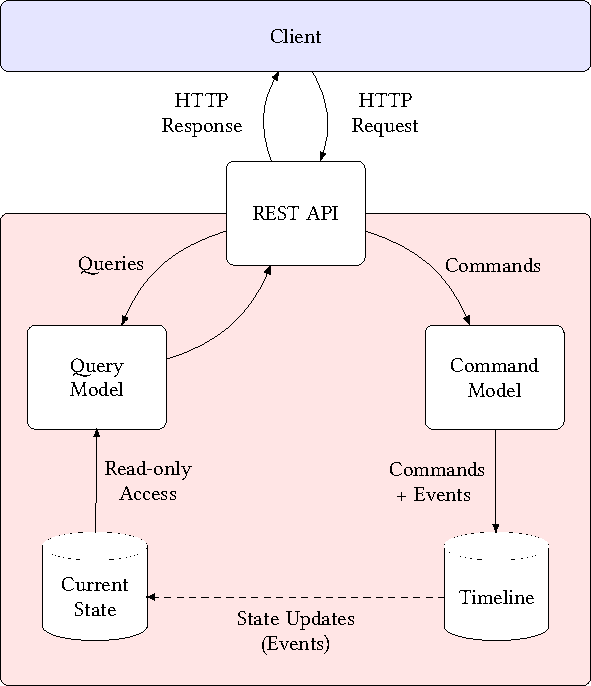
\includegraphics[width=0.5\textwidth]{../illustrations/rest.pdf}
	\caption{
		The figure is a schematic illustration of our prototype.
		A client sends HTTP requests to the REST API and receives a 
		response. The API maps these requests to application commands 
		and queries.
	}
	\label{fig:rest}
\end{figure}

\subsection{The Application Interface}
\begin{table}
\footnotesize
\centering
\begin{tabular}{c | l | l | l | l | l }
 & Semantics 	& Method	 	& Resource	& Payload			& Application Mapping \\
\hline \hline
Q & List all products 		& \cmd{GET} 			& \cmd{/products}	& & \cmd{getProducts()}  				 \\
Q & List details of product 	& \cmd{GET} 			& \cmd{/products/:id}	& & \cmd{getProduct(:id)} 				  \\
 && & & &  \\
Q & Display items in cart 		& \cmd{GET}			& \cmd{/cart}		& & \cmd{getCart()}  				 \\
C & Empty shopping cart 		& \cmd{DELETE}			& \cmd{/cart/}  	& & \cmd{emptyCart()}  \\
C & Put item in cart 		& \cmd{POST}			& \cmd{/cart/:id}	&  \cmd{\{qty: 1\}} & \cmd{addToCart(:id, :qty)} \\
C & Update item quantity  		& \cmd{PUT}			& \cmd{/cart/:id}	&  \cmd{\{qty: 5\}} & \cmd{updateQty(:id, :qty)} \\
C & Remove item from cart 		& \cmd{DELETE}			& \cmd{/cart/:id}	& & \cmd{removeFromCart(:id)} 				  \\
 & & & & \\
C & Place order 			& \cmd{POST}			& \cmd{/order}	& 				& 1) \cmd{fetchCurrencyRate()}  \\
		& & 			& 		& & 2) \cmd{createOrder()} \\
		& & 			& 		& & 2) \cmd{sendConfirmation()} \\
\end{tabular}\\
\caption{The table lists resources and operations of the online shop. 
The REST interface maps and distributes HTTP requests to system commands
(C) and queries (Q). Two application commands yield side effects: 
\cmd{fetchCurrencyRate()} is an external query and returns data,
\cmd{sendConfirmation()} is an external command, which triggers the
transmission of a mail message.
}
\label{tbl:rest-shop}
\end{table}


Representational State Transfer (REST) is a resource-oriented style of architecture~\cite{Fielding2000},
which corresponds to the principles of the World Wide Web. This architectural 
style was introduced by Roy Fielding and has gained popularity in recent years. 
Today, many large web services -- Twitter, Facebook, or Google, for example -- 
utilize REST to provide APIs over the web.
There are numerous reasons for this. Among them is that REST promotes statelessness -- 
each request to an API holds everything needed to fulfill it. The server does not 
hold session state, which makes it easier to build scalable systems.
The most common application of REST is the usage of HTTP to provide web services: 
Uniform Resource Identifiers (URIs) are used as identifiers when accessing 
resources, HTTP methods are used as verbs to operate on these resources. 
The HTTP verbs possess a clearly specified semantics \cite{RFC2616}: 
\texttt{GET} and \texttt{HEAD}, for example, are considered safe and should not 
mutate state, whereas e.g. \texttt{POST}, \texttt{PUT}, or \texttt{DELETE} may 
change state.

Our prototype provides a RESTful API to clients. We chose to use REST, since it 
already provides a clear segregation in queries (safe verbs) and commands (not 
safe verbs). This inherent segregation works in favor of our CQRS architecture. 
The API can be accessed using e.g. a browser or command-line tools, such as cURL 
or wget. 
Table \ref{tbl:rest-shop} lists all resources which are exposed over REST and 
the HTTP verbs which can be used on them. 
%
A shopping cart in a REST architecture is typically modelled as one resource 
\texttt{/cart}, which can be updated using the \texttt{PUT} verb. But in HTTP, 
\texttt{PUT} possesses the semantics of replacing a resource: 
``\emph{The PUT method requests that the enclosed entity be stored under the
supplied Request-URI. [\dots{}] the enclosed entity SHOULD be considered as a 
modified version of the one residing on the origin server.}'' \cite{RFC2616}.
%
This can conflict with retroaction.
As described in Section \ref{sec:command-semantics}, the semantics of commands 
can lead to unintended reversals of retroaction. Here, a \texttt{PUT} command 
overwrites an entire resource each time it is invoked. Thus, retroactively 
injected updates of the cart would be annihilated by the next cart update in 
the timeline.
As a consequence, we modelled individual items in the cart as separate 
resources. By applying \cmd{POST}, items can be added to the cart. Their 
quantity can be updated using \cmd{PUT}.
By applying \cmd{DELETE} on individual cart item resources, they can be removed 
from the cart.

Furthermore, we provide a command with the semantics of emptying the shopping
cart. The operation \texttt{DELETE /cart} can be used to empty the cart. 
This command will annihilate previous \cmd{addToCart()} commands (and events), 
but in this case the semantics is different: delete all items from the cart.
Thus, annihilating prior events is an intended consequence.

In our prototype, HTTP requests are sent to the REST API. This interface 
contains a thin logic layer, it maps and distributes requests to system 
commands and queries.
Figure \ref{fig:rest} depicts a schematic illustration of this process. 
The mapping of application commands and requests is visible in Figure 
\ref{tbl:rest-shop}. In order to fulfill e.g. the \cmd{POST /order} command, 
a \cmd{fetchCurrencyRate()}, a \cmd{CreateOrder()}, and a \cmd{SendConfirmation()} 
command are issued subsequently by the API. 
This is done sequentially; the runtime engine waits for each command to finish 
its execution.
After each command returns, the runtime engine checks if the command succeeded. 
If it did, the command and the resulting event are persisted to the timeline and
the next command in the series is processed. If the command failed, the commands 
in the series will not be processed further. But the commands are still persisted 
to the timeline, in order to enable later replays. 
The following figure depicts a possible course of computation for the mentioned 
series. First, the currency is fetched, then the order creation is attempted. 
This fails and hence the subsequent \cmd{sendConfirmation()} command is not 
processed (highlighted in yellow). It is persisted to the timeline though and 
can be recomputed in a replay.

\begin{figure}[h!]
	\centering
	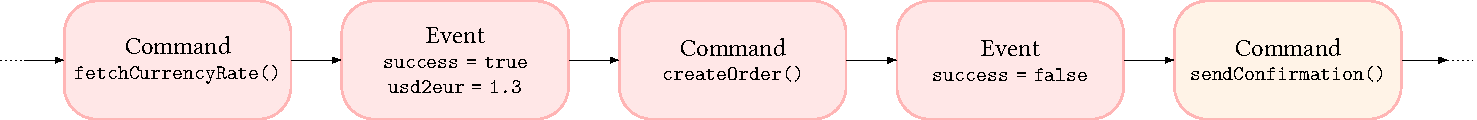
\includegraphics[width=1.0\textwidth]
		{../illustrations/projections3.pdf}

	%\caption{ }
	%\label{fig:projections3}
\end{figure}

Listing \ref{lst:implcp} displays a relevant excerpt from the runtime engine, 
which depicts this process.
The \cmd{fetchCurrencyRate()} has a purely reading side effect (an external 
query). It fetches current currency exchange rates and persists them to the 
system state. These exchange rates are used during the calculation of an order 
price. The \cmd{sendConfirmation()} command triggers a purely writing side 
effect (an external command) which sends irrevocable confirmation messages 
via mail.

\begin{lstlisting}[
	style=styled 
	, caption=Shortened and simplified excerpt from the REST API.
	, label = lst:implcp
]
restAPI.commands = function(request) {
	/* map HTTP requests to commands */
	if (request === "POST /order) {
		var commands = [
			"fetchCurrencyRate(request, state)",
			"createOrder(request, state)",
			"sendConfirmation(request, state)"
		];

		// 1) invoke each command in the series sequentially.
		//    this enforces a causal order by waiting for each 
		//    command to terminate, before the next is invoked.
		// 2) for each comand, calculate event from state changes
		      and persist command + event.
		// 4) publish events to query model(s).
		runtimeEngine.processCommands(commands, request);
	}
}
\end{lstlisting}

\subsection{Command Implementation}
Commands are implemented as modifying the system state object. The runtime 
engine generates an event after a command has been executed. This event
captures the change to the prior state object.
%
Within commands, the programmer annotates which state properties were read 
during the computation. 
Modified state properties are automatically captured by the runtime engine.
This enables the runtime engine to track causalities between events (Section 
\ref{sec:dependent}).
%
Thus, if we e.g. remove a \evt{ProductAddedToCart} event from the timeline, 
subsequent causally dependent events (e.g. \cmd{PlacedOrder}) can be 
automatically removed (or replayed) as well.
Listing \ref{lst:two} depicts two command implementations.

\begin{lstlisting}[
	style=styled, 
	caption={Two examples of online shop commands.},
	label = lst:two
]
/* command, which adds items to the cart */
commands.addToCart = function(request, state){
	/* extract parameters from the HTTP request, update state  */
	var productId = request.params.productId;
	var quantity = request.params.qty;
	state.cart[productId] = quantity;

	return {
		success: true,
		newState: state,
		read: []
	};
}

/* command, which places an order */
commands.placeOrder = function(request, state){
	var order = { items: state.cart, sum: ... }
	state.orders.push(order);
	state.cart = {};

	return {
		success: true,
		newState: state,
		read: []
	};
}
\end{lstlisting}

\subsection{Events}
The already mentioned JSON Patches serve as the data format for events.
Events in our implementation are created automatically by the runtime engine.
We implemented this feature using an open source library\footnote[1]{\href{https://github.com/Starcounter-Jack/JSON-Patch}{https://github.com/Starcounter-Jack/JSON-Patch}},
which offers the possibility to output changes to objects in the form of a 
JSON Patch. For this, it utilizes the \mbox{\texttt{Object.observe()}} feature 
from ECMAScript 2016 (ES7), the most recent specification of the JavaScript 
language. This feature provides a mean for recording changes to an 
object\footnote[2]{\href{https://developer.mozilla.org/de/docs/Web/JavaScript/Reference/Global_Objects/Object/observe}{https://developer.mozilla.org/de/docs/Web/JavaScript/Reference/Global\_Objects/Object/observe}}.
We applied this to record modifications of the system state object.
This enables us to automatically generate the patch after a command has been 
processed. Together with event tags, state properties which were used, and a 
preliminary id (explained later in this section), this patch forms the event.
After the event has been created, it is persisted to the timeline together
with the command. The event is furthermore published to the query model(s).
%
\mbox{Listing \ref{lst:patches}} displays the patches of some events, which were
automatically generated by the prototype runtime engine.

\begin{lstlisting}[
	style = styled, 
	caption = {Events in the form of JSON Patches, from our prototype. They depict modifications of the system state object.},
	label = lst:patches
]
/* add product id 172 to the "state.cart" object with quantity 1 */
[ { "op": "add", "path": "/cart/172", "value": 1 } ]

/* update the quantity of the product "state.cart[172]" */
[ { "op": "replace", "path": "/cart/172", "value": 3 } ]

/* add an object to "state.orders" array and remove it from cart */
[{
	"op": "add",
	"path": "/orders/-",
	"value": {
		"timestamp": 1458061070313,
		"content": { "172": 3 }
	}
}, 
{
	"op": "remove",
	"path": "/cart/172"
}]
\end{lstlisting}

\subsection{Queries}
Queries are sent as HTTP requests to the REST API, using safe HTTP verbs. 
The thin logic layer in the API then maps the requests to a query model, which 
responds with the state visible in the model.
The method in the following listing returns the shopping cart content, when queried.

\begin{lstlisting}[style=styled]
queryModel.getCart = function(request, state) {
	request.send(state.cart);
}
\end{lstlisting}

We apply CQRS here: The query model is decoupled from the command model and 
there might exist a multitude of replicated query model instances which
could be used to conduct e.g. load balancing. 
As examined in Section \ref{sec:cqrs}, this results in an eventually consistent 
behavior of queries.
Listing \ref{lst:rr} displays an excerpt of this routing, using a simple round 
robin algorithm.

\begin{lstlisting}[
	style=styled, 
	caption=Simplified excerpt from the query routing in the API.,
	label= lst:rr
]
restAPI.queries = (request, state) {
	var roundRobin = ++roundRobin % queryModels.length;
	if (request === "GET /cart") {
		queryModel[roundRobin].getCart(request, state));
	}
	// ...
}
\end{lstlisting}

\subsection{Preliminary Command IDs}
\label{sec:prelim}
Following our argumentation from Section \ref{sec:return-values}, we implement 
commands in a way that the HTTP request receives a preliminary command id as an
immediate response. 
This preliminary id can be used by clients to ensure that queries are only 
fulfilled, if the result of a certain command is visible in the query model. 
%
We propose a solution which ties in with the principles behind REST.
Commands in our prototype return the HTTP status code ``\texttt{202 Accepted}'' 
to indicate that the request has been accepted and will be processed
asynchronously. The preliminary id is returned as the payload:

\begin{lstlisting}[style=styled]
HTTP/1.1 202 Accepted 
Content-Type: application/json;charset=utf-8
...

{ "preliminary_id": 533 }
\end{lstlisting}

Queries can be restricted to a certain preliminary id. If this id is not yet 
visible in the query model, the query is rejected. To achieve this, we utilize 
the \texttt{If-Match} field available in HTTP/1.1 as a mean for conditional HTTP 
requests. The specification matches our use case:
``\emph{The 'If-Match' header field makes the request method conditional on
the recipient origin server either having at least one current representation of 
the target resource [\dots{}]}'' \cite{RFC7232}.
%
Listing \ref{lst:testscript} depicts a simple script which we used to test our 
prototype (among other test scripts). The script sends two succeeding HTTP 
requests: a command (line 6-10) and a query (line 14-17). The query is sent as a 
conditional request using the preliminary id which was returned by the prior command.

\pagebreak

\begin{lstlisting}[
	style = styled,
	numbers = left,
	numberstyle = \footnotesize,
	caption = {Simple Test Script for our Prototype.},
	label = lst:testscript
]
#!/bin/ksh
URI=http://localhost:8000

# add item to cart
PRELIMINARY_ID=$(
	curl	-X POST                                     \
		    -H "Content-Type: application/json"         \
		    -d '{ "qty": 3 }'                           \
		    $URI/cart/724                               \
		    | grep -o '[0-9]*'
)

# list items in cart
curl    -v -X GET                                   \
        -H 'Accept: text/plain'                     \
        -H "If-Match: $PRELIMINARY_ID"              \
        $URI/cart
\end{lstlisting}

The command adds a product to the cart and obtains a preliminary id. The HTTP 
exchange looks roughly like in the following listing. Lines starting with 
``\cmd{>}'' indicate a HTTP request from the client to the server, lines 
starting with ``\cmd{<}'' mark the response.

\begin{lstlisting}[style=styled]
> POST /cart/724 HTTP/1.1
> Content-Type: application/json;charset=utf-8
> ...
> 
> { "qty" : 3 }

< HTTP/1.1 202 Accepted 
< Content-Type: application/json;charset=utf-8
< ...
<
< { "preliminary_id": 1458171779004 }
\end{lstlisting}

The second HTTP request (from Listing \ref{lst:testscript}), obtains the content 
of the shopping cart. In accordance to the HTTP/1.1 specification for conditional 
requests, the server returns ``\cmd{304 Not Modified}'' if the condition evaluated 
to false and ``\cmd{200 OK}'' if it succeeded \cite{RFC7232}.
The following listing depicts this rejection (line 5-9) and the alternative response 
(line 13-19).

\begin{lstlisting}[
	style=styled, 
	numbers = left,
	numberstyle = \footnotesize
]
> GET /cart HTTP/1.1
> If-Match: 1458171779004
> ...

< HTTP/1.1 304 Not modified
< Content-Type: application/json;charset=utf-8
< ...
<
< { "visible" : false }

OR

< HTTP/1.1 200 OK
< Content-Type: application/json;charset=utf-8
< ...
<
< [ 
< 	{ "product1" : { "title": "Lorem Ipsum", "price": 99 }  }
< ]
\end{lstlisting}


\subsection{Retroactive Use Cases}
In this section we describe some of the use cases for retroaction, which 
can be applied to our prototype. %which we implemented in the prototype.

\subsubsection{History-aware Algorithms}
Through the programming model which we described, the history of the application 
is exposed to commands. This can be utilized to create history-aware algorithms.
An example for this is a \cmd{PlaceOrder} command which calculates an order 
discount based on previous orders by this customer. Listing \ref{lst:impl-po1}
depicts the commands' implementation.
First, a branch of the timeline is created, then all events tagged with 
\evt{placed-order} are searched for. Next, these events are examined in order 
to compute a discount for the current order.

\begin{lstlisting}[
	  style = styled 
	, caption = {When placing an order, a discount based on previous orders is calculated.}
	, label = lst:impl-po1
]
commands.placeOrder = function(request, state) {
	/* 'big bang' is a pre-defined tag of the runtime engine which
	   refers to the start of the timeline. */
	var b = retroactive.createBranch("big bang");

	/* find all events tagged with 'placed-order' */
	var orderEvents = b.getEvents(["placed-order"]);

	var allOrdersAmount = 0;
	for (var o in orderEvents) {
		/* get the system state object at the point of this event 
		   in the timeline */
		allOrdersAmount += orderEvents[o].getState().totalAmount;
	}

	var discount = 0;
	if (allOrdersAmount > 1000) discount = 0.1;      /* 10% */
	else if (allOrdersAmount > 100) discount = 0.05; /*  5% */

	var order = {
		items: ...,
		totalAmount: ... * discount
	};
	state.orders.push(order);

	return { success: ..., newState: ..., read: ... };
}
\end{lstlisting}


\subsubsection{Partial Replay with Control of Side Effects}
The concept of partial replays allows for control of the side effects in a 
replay (Section \ref{sec:replaying-se}).
It is possible to either reuse prior results or reinvoke them and continue 
the processing with these new results. As we described it, the shop fetches 
current currency exchange rates before creating an order. A use case is to 
replay the shop timeline and reprocess each \cmd{fetchCurrencyRate()}.
In such a replay, the shop fetches each currency exchange rate from an 
external web service again. Each causally dependent command (\cmd{placeOrder()} 
in this case) will then be reprocessed with the new result.
In order to prevent confirmations from being sent out again, we suppress them.
In this case, suppressing the invocation means that we reuse the event from the 
last \cmd{sendConfirmation()} invocation (if an event is available).

\begin{lstlisting}[
	  style = styled 
	, caption = {Partial Replay Example}
	, label = lst:impl-po2
]
/* newly compute the events in this array, instead of reusing the 
   already persisted ones */
var recomputeCommands = [ "fetch-currency-rate" ];

/* for the tags in the array use the persisted events instead of 
   newly invoking the command */
var reuseEvents= [ "confirmation-mail" ];

/* normal event replay, but for the supplied 'newlyComputeEvents'
   array the belonging command is newly invoked. Events which
   possess a causal relationship to the newly computed ones are
   recomputed as well, as long as they are not specified in the
   'reuseEvents' array. */
var b = createBranch("big bang");
b.partialReplay({ recompute: recomputeCommands, reuse: reuseEvents });
\end{lstlisting}

In the code above \emph{all} \cmd{fetchCurrencyRate()} commands and the direct 
and indirect causally related events are reprocessed. 
But it would also have been possible to reprocess just a single specific 
\cmd{fetchCurrencyRate()} and its causally related events. 
This can be achieved through the usage of unique (or appropriately fine-grained)
tags within the commands. These tags can then be filtered for in a later replay.

\subsubsection{Alternate Command Behavior}
We can adapt the above code to evaluate how different currency exchange rates
would have affected the state. 
To achieve this, we exchange the \cmd{fetchCurrencyRate()} command in a branch. 
Instead a function which returns hypothetical exchange rates from a fixed list
is used. Then a replay of the relevant commands is conducted. Next, the resulting 
state can be accessed for further analysis:

\begin{lstlisting}[style=styled]
var experimentalRatesFn = function(request, state) {
	/* use this fixed currency rate for the new processing */
	state.currencyRates = { eur2usd: 1.13 };

	return { 
		success: true, 
		newState: state, 
		read: [] 
	};
}

var someCommand = function(request, state) {
	b.createBranch("big bang");
	b.changeCommandFunction("fetchCurrencyRate", 
	                        "experimentalRatesFn");
	
	b.partialReplay({ 
		recompute: ["fetch-currency"],
		reuse: ["confirmation-mail"]
	});

	var experimentalOrders = b.getState().orders;

	// further processing
	// ...

	return { success: true, newState: ..., read: ... };
}
\end{lstlisting}

\subsubsection{Observe Alternate States}
We implemented a feature which allows for displaying how the orders would have 
been different, if customers would not have removed any products from their cart.
For this, a branch is created and all events tagged with \evt{product-removed-from-cart} 
are deleted from it. Next, a replay of commands tagged with \cmd{place-order} 
is conducted.

\begin{lstlisting}[style=styled]
commands.calculatePossibleOrders = function(request, state) {
	var b = retroactive.createBranch("big bang");

	/* supplying true would remove all causally dependent 
	   "place-order" events as well. */
	b.deleteEvents("product-removed-from-cart", false);

	/* only these commands (and the ones which read state modified 
	   by these ones) are recomputed, for other commands the events 
	   are reused */
	var recomputeCommands = [ "place-order" ];

	var b = createBranch("big bang");
	var reuseEvents = ["confirmation-mail"];
	b.partialReplay({ 
		recompute: recomputeCommands, 
		reuse: reuseEvents 
	});

	var branchState = b.getState();
	state.whatifOrders = branchState.orders;

	return {
		newState: state,
		success: true,
		read: []
	};
}
\end{lstlisting}

The result from this analysis is saved to the state property \cmd{state.whatifOrders} 
and subsequently persisted to the timeline as an event, by the runtime engine.
The query model(s) eventually receive the events as state updates. Then the 
results are visible in the query model. They are exposed to the clients through 
a query:

\begin{lstlisting}[style=styled]
queries.getPossibleOrders = function(request, state) {
	return state.whatifOrders;
}
\end{lstlisting}

\subsubsection{Retroaction for Optimization}
It is possible to use the application's history for optimization or adaption of
the application's current behavior. This is the use case which we described in 
Chapter \ref{chp:related-work} as history-aware and self-improving algorithms.
%
Concerning the online shop, this section described the implementation of a 
history-aware discount algorithm. But it is also possible to use the system's 
history for evaluating experimental -- and possibly better performing -- 
algorithms. This can be achieved by replaying commands from the timeline
with a different command processing implementation. The resulting state can 
then be used for comparison against the current state of the timeline -- and 
thus against the current discount algorithm. 
Next, we can adapt the future application behavior based on these insights.

To achieve this, we create a command which creates a branch, exchanges the 
\mbox{\cmd{placeOrder()}} command implementation, conducts a replay, and 
compares the branch state against the application state. Based on this result, 
the current command function can then be exchanged.

\begin{lstlisting}[style=styled]
commands.tags.placeOrder = ["place-order"];
commands.experimentalFn = function(request, state) { ... }

commands.optimizeAlgorithm = function(request, state) {
	var b = createBranch("beginning of timeline");
	b.changeCommandFunction("placeOrder", "experimentalFn");
	b.partialReplay({ recompute: [ "place-order" ] });

	/* compare branch state against current state */
	var branchState = b.getState();
	if (...) {
		/* exchange command function in ongoing timeline */
		changeCommandFunction("commands.placeOrder", 
                          "commands.experimentalFn");
	}

	return ...;
}
\end{lstlisting}

In order to compare different processing implementations against each other,
it has to be clear that the differences after a replay have occurred due to
the different command processing implementation. 
Therefore a deterministic command replay needs to be ensured. If commands are 
processed in a different order, the differences might as well be due to this 
indeterminism. Hidden causalities need to be taken into account as well, 
otherwise one could mistakenly attribute differences in the outcome to the 
different command processing, although hidden causalities or side effects 
could be responsible as well.

\subsubsection{Iterate Towards Target State}
A further use case is to define a target state and modify the past until we 
reach it. We can determine if we get from a specified start state to a defined 
target state by applying subsequent, iterative modifications.
This feature is especially interesting for problems where modifications have 
to be ``played through'' and cannot be trivially calculated. 
%
For example, the online shop could have a complex algorithm, which calculates
price increases each time an order is placed.
Lets say this calculation is complex. It depends on the state of the system at 
the time when an order is placed and takes the number of similar recent product 
orders into account. 
If we want to find out how much more orders would have had to be placed for
the current price of a product to reach a specified state, we can retroactively
insert orders until we reach our target state.

But this strategy is not limited to insertion or removal operations of commands 
and events. It can also be applied to the command processing implementation, to 
determine how the logic needs to be modified to reach a certain state. This 
process then yields the necessary modifications.
In general, this can be beneficial for a lot more cases, where the behavior of 
the application over time needs to be considered or is time-dependent.
We imagine that this feature allows for novel debugging schemes and bug fixes. 

\subsection{Prototype Limitations}
A limitation of our prototype is that if one command in the series fails, the 
series will not be executed further. This limits the expressiveness, since 
rollbacks of commands in the series are not possible.
Additionally, it is not possible to issue a hierarchical series, where parts of
the series can be executed independent of each other. 

The annotation, which state properties were used for the computation of a
state change, is cumbersome and could probably be done by an underlying 
runtime engine. We are confident that this could be achieved through source 
code analysis, by observing which state properties are accessed and modified.
Another option is to use explicit getter and setter methods when accessing 
properties of the state object.
Such methods can record the access of state properties as well.

Last, we have by far not exhausted the possibilities for retroactive operations,
which the API could expose. For example, forward deleting all events from a certain
branching point could be helpful, if the objective is to append simulated
events from a certain point on. This is not possible with our described
prototype, but could certainly be implemented. We have restrained our description
to a basic set of operations to keep the concept simple and comprehensible.



\section{Summary}
This chapter demonstrated the practical applicability of the concepts described 
in Chapter \ref{chp:concept}. In Section \ref{sec:arch:arch-unified}, we 
described two contrasting architectural modifications for event-sourced systems 
following a CQRS style of architecture, as means to utilize retroaction: a 
unified architecture and a plug-in architecture.
%
This chapter outlined a programming model for the unified architecture. A 
prototypical implementation using the scenario of an online shop was described. 
We demonstrated how issues of retroactive systems can be addressed (e.g. by 
constraining possible modifications) and which new problems emerge from the 
application of our ideas (e.g. retroaction-aware programming).
%
Furthermore, the central role which the delta encoding of events poses to 
retroaction has been highlighted. Our programming model provides the ability 
to access and manipulate the application's state history in a single environment. 
This enables a variety of possibilities, such as history-aware algorithms and 
novel debugging schemes.
Developers can use the application's data structures, functions, and libraries 
in the retroactive code. They can conduct analyses of the application's history, 
explore alternate branches, or create history-aware algorithms.
